% LR constraints - Drawing and filling with arcs and Bezier curves
% Author: Henri Menke
\documentclass[tikz, border=10pt]{standalone}
%%%<
\usepackage{verbatim}
%%%>
\begin{comment}
:Title: LR constraints - Drawing and filling with arcs and Bezier curves
:Tags: Diagrams;Styles;Coordinate calculations;Computer Science
:Author: Henri Menke
:Slug: draw-fill-bezier-curves

We use TikZ to reproduce a diagram  seen in an article
"The Left-Right Planarity Test" by Ulrik Brandes.

At first we adjust the bounding box by hand, because the control points
of the bezier curves exceed the limits of the visible drawing.

The code was written by Henri Menke and published on TeX.SE.
\end{comment}
\usetikzlibrary{calc}
\tikzset{
    vertex/.style = {
        circle,
        fill      = black,
        outer sep = 2pt,
        inner sep = 1pt,
    }
}
\begin{document}
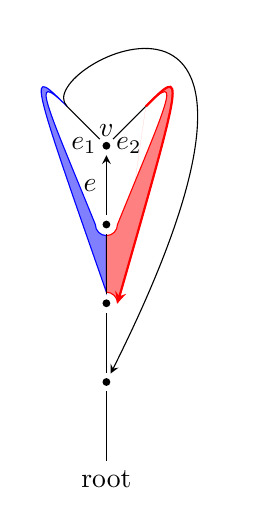
\begin{tikzpicture}[>=stealth]
  % We need to adjust the bounding box manually
  % as the control points enlarge it.
  \path[use as bounding box] (-1,-0.5) rectangle (1.5,5.5);

  \coordinate (o) at (0,0);
  \node[below] at (o) {root};
  \draw node[vertex] (a) at (0,1) {};
  \draw node[vertex] (b) at (0,2) {};
  \draw node[vertex] (c) at (0,3) {};
  \draw node[vertex] (d) at (0,4) {};
  \node[above] at (d) {$v$};

  \draw (d) node[left] {$e_1$} -- (-0.5,4.5);
  \filldraw[draw=blue, fill=blue!50]
    (-0.5,4.5) .. controls (-1,5) and (-0.75,4.5) .. ($(c)+(180:4pt)$)
    arc[start angle=180, end angle=270, radius=4pt]
    -- ($(b)+(90:4pt)$) .. controls (-1,5) .. (-0.5,4.5);
  \draw (d) node[right] {$e_2$} -- (0.5,4.5);
  \filldraw[draw=red, fill=red!50]
    (0.5,4.5) .. controls (1,5) and (0.75,4.5) .. ($(c)+(0:4pt)$)
    arc[start angle=0, end angle=-90, radius=4pt]
    -- ($(b)+(90:4pt)$) arc[start angle=90, end angle=0, radius=4pt]
    ($(b)+(0:4pt)$) .. controls (1,5) .. (0.5,4.5);
  \draw[red, thick, ->] (0.5,4.5) .. controls (1,5) .. ($(b)+(0:4pt)$);
  \draw[->] (-0.5,4.5) .. controls (-1,5) and (3,7) .. (a);

  \draw[->] (o) -- (a) (a) -- (b) (b) -- (c) (c) -- node[left] {$e$} (d);
\end{tikzpicture}
\end{document}